% Options for packages loaded elsewhere
\PassOptionsToPackage{unicode}{hyperref}
\PassOptionsToPackage{hyphens}{url}
%
\documentclass[
]{article}
\usepackage{amsmath,amssymb}
\usepackage{lmodern}
\usepackage{iftex}
\ifPDFTeX
  \usepackage[T1]{fontenc}
  \usepackage[utf8]{inputenc}
  \usepackage{textcomp} % provide euro and other symbols
\else % if luatex or xetex
  \usepackage{unicode-math}
  \defaultfontfeatures{Scale=MatchLowercase}
  \defaultfontfeatures[\rmfamily]{Ligatures=TeX,Scale=1}
\fi
% Use upquote if available, for straight quotes in verbatim environments
\IfFileExists{upquote.sty}{\usepackage{upquote}}{}
\IfFileExists{microtype.sty}{% use microtype if available
  \usepackage[]{microtype}
  \UseMicrotypeSet[protrusion]{basicmath} % disable protrusion for tt fonts
}{}
\makeatletter
\@ifundefined{KOMAClassName}{% if non-KOMA class
  \IfFileExists{parskip.sty}{%
    \usepackage{parskip}
  }{% else
    \setlength{\parindent}{0pt}
    \setlength{\parskip}{6pt plus 2pt minus 1pt}}
}{% if KOMA class
  \KOMAoptions{parskip=half}}
\makeatother
\usepackage{xcolor}
\IfFileExists{xurl.sty}{\usepackage{xurl}}{} % add URL line breaks if available
\IfFileExists{bookmark.sty}{\usepackage{bookmark}}{\usepackage{hyperref}}
\hypersetup{
  pdftitle={Modern Applyed Statistics(Chap 11)},
  hidelinks,
  pdfcreator={LaTeX via pandoc}}
\urlstyle{same} % disable monospaced font for URLs
\usepackage[margin=1in]{geometry}
\usepackage{color}
\usepackage{fancyvrb}
\newcommand{\VerbBar}{|}
\newcommand{\VERB}{\Verb[commandchars=\\\{\}]}
\DefineVerbatimEnvironment{Highlighting}{Verbatim}{commandchars=\\\{\}}
% Add ',fontsize=\small' for more characters per line
\usepackage{framed}
\definecolor{shadecolor}{RGB}{248,248,248}
\newenvironment{Shaded}{\begin{snugshade}}{\end{snugshade}}
\newcommand{\AlertTok}[1]{\textcolor[rgb]{0.94,0.16,0.16}{#1}}
\newcommand{\AnnotationTok}[1]{\textcolor[rgb]{0.56,0.35,0.01}{\textbf{\textit{#1}}}}
\newcommand{\AttributeTok}[1]{\textcolor[rgb]{0.77,0.63,0.00}{#1}}
\newcommand{\BaseNTok}[1]{\textcolor[rgb]{0.00,0.00,0.81}{#1}}
\newcommand{\BuiltInTok}[1]{#1}
\newcommand{\CharTok}[1]{\textcolor[rgb]{0.31,0.60,0.02}{#1}}
\newcommand{\CommentTok}[1]{\textcolor[rgb]{0.56,0.35,0.01}{\textit{#1}}}
\newcommand{\CommentVarTok}[1]{\textcolor[rgb]{0.56,0.35,0.01}{\textbf{\textit{#1}}}}
\newcommand{\ConstantTok}[1]{\textcolor[rgb]{0.00,0.00,0.00}{#1}}
\newcommand{\ControlFlowTok}[1]{\textcolor[rgb]{0.13,0.29,0.53}{\textbf{#1}}}
\newcommand{\DataTypeTok}[1]{\textcolor[rgb]{0.13,0.29,0.53}{#1}}
\newcommand{\DecValTok}[1]{\textcolor[rgb]{0.00,0.00,0.81}{#1}}
\newcommand{\DocumentationTok}[1]{\textcolor[rgb]{0.56,0.35,0.01}{\textbf{\textit{#1}}}}
\newcommand{\ErrorTok}[1]{\textcolor[rgb]{0.64,0.00,0.00}{\textbf{#1}}}
\newcommand{\ExtensionTok}[1]{#1}
\newcommand{\FloatTok}[1]{\textcolor[rgb]{0.00,0.00,0.81}{#1}}
\newcommand{\FunctionTok}[1]{\textcolor[rgb]{0.00,0.00,0.00}{#1}}
\newcommand{\ImportTok}[1]{#1}
\newcommand{\InformationTok}[1]{\textcolor[rgb]{0.56,0.35,0.01}{\textbf{\textit{#1}}}}
\newcommand{\KeywordTok}[1]{\textcolor[rgb]{0.13,0.29,0.53}{\textbf{#1}}}
\newcommand{\NormalTok}[1]{#1}
\newcommand{\OperatorTok}[1]{\textcolor[rgb]{0.81,0.36,0.00}{\textbf{#1}}}
\newcommand{\OtherTok}[1]{\textcolor[rgb]{0.56,0.35,0.01}{#1}}
\newcommand{\PreprocessorTok}[1]{\textcolor[rgb]{0.56,0.35,0.01}{\textit{#1}}}
\newcommand{\RegionMarkerTok}[1]{#1}
\newcommand{\SpecialCharTok}[1]{\textcolor[rgb]{0.00,0.00,0.00}{#1}}
\newcommand{\SpecialStringTok}[1]{\textcolor[rgb]{0.31,0.60,0.02}{#1}}
\newcommand{\StringTok}[1]{\textcolor[rgb]{0.31,0.60,0.02}{#1}}
\newcommand{\VariableTok}[1]{\textcolor[rgb]{0.00,0.00,0.00}{#1}}
\newcommand{\VerbatimStringTok}[1]{\textcolor[rgb]{0.31,0.60,0.02}{#1}}
\newcommand{\WarningTok}[1]{\textcolor[rgb]{0.56,0.35,0.01}{\textbf{\textit{#1}}}}
\usepackage{graphicx}
\makeatletter
\def\maxwidth{\ifdim\Gin@nat@width>\linewidth\linewidth\else\Gin@nat@width\fi}
\def\maxheight{\ifdim\Gin@nat@height>\textheight\textheight\else\Gin@nat@height\fi}
\makeatother
% Scale images if necessary, so that they will not overflow the page
% margins by default, and it is still possible to overwrite the defaults
% using explicit options in \includegraphics[width, height, ...]{}
\setkeys{Gin}{width=\maxwidth,height=\maxheight,keepaspectratio}
% Set default figure placement to htbp
\makeatletter
\def\fps@figure{htbp}
\makeatother
\setlength{\emergencystretch}{3em} % prevent overfull lines
\providecommand{\tightlist}{%
  \setlength{\itemsep}{0pt}\setlength{\parskip}{0pt}}
\setcounter{secnumdepth}{-\maxdimen} % remove section numbering
\ifLuaTeX
  \usepackage{selnolig}  % disable illegal ligatures
\fi

\title{Modern Applyed Statistics(Chap 11)}
\author{}
\date{\vspace{-2.5em}}

\begin{document}
\maketitle

\hypertarget{library-package}{%
\subsection{Library Package}\label{library-package}}

\begin{Shaded}
\begin{Highlighting}[]
\FunctionTok{library}\NormalTok{(MASS)}
\end{Highlighting}
\end{Shaded}

\hypertarget{data-input}{%
\subsection{Data input}\label{data-input}}

\begin{Shaded}
\begin{Highlighting}[]
\CommentTok{\# 1. Iris data}
\FunctionTok{data}\NormalTok{(iris3)}
\FunctionTok{head}\NormalTok{(iris)}
\end{Highlighting}
\end{Shaded}

\begin{verbatim}
##   Sepal.Length Sepal.Width Petal.Length Petal.Width Species
## 1          5.1         3.5          1.4         0.2  setosa
## 2          4.9         3.0          1.4         0.2  setosa
## 3          4.7         3.2          1.3         0.2  setosa
## 4          4.6         3.1          1.5         0.2  setosa
## 5          5.0         3.6          1.4         0.2  setosa
## 6          5.4         3.9          1.7         0.4  setosa
\end{verbatim}

\begin{Shaded}
\begin{Highlighting}[]
\CommentTok{\# 2. Leptograpsus variegatus crabs data}
\FunctionTok{data}\NormalTok{(}\StringTok{"crabs"}\NormalTok{)}
\FunctionTok{head}\NormalTok{(crabs)}
\end{Highlighting}
\end{Shaded}

\begin{verbatim}
##   sp sex index   FL  RW   CL   CW  BD
## 1  B   M     1  8.1 6.7 16.1 19.0 7.0
## 2  B   M     2  8.8 7.7 18.1 20.8 7.4
## 3  B   M     3  9.2 7.8 19.0 22.4 7.7
## 4  B   M     4  9.6 7.9 20.1 23.1 8.2
## 5  B   M     5  9.8 8.0 20.3 23.0 8.2
## 6  B   M     6 10.8 9.0 23.0 26.5 9.8
\end{verbatim}

\newpage

\hypertarget{visualization-methods}{%
\subsection{1. Visualization Methods}\label{visualization-methods}}

\hypertarget{principal-component-analysis}{%
\subsubsection{1-1) Principal component
analysis}\label{principal-component-analysis}}

\begin{Shaded}
\begin{Highlighting}[]
\CommentTok{\# Iris Data}
\NormalTok{ir }\OtherTok{\textless{}{-}} \FunctionTok{rbind}\NormalTok{(iris3[,,}\DecValTok{1}\NormalTok{], iris3[,,}\DecValTok{2}\NormalTok{], iris3[,,}\DecValTok{3}\NormalTok{])}
\NormalTok{ir.species }\OtherTok{\textless{}{-}} \FunctionTok{factor}\NormalTok{(}\FunctionTok{c}\NormalTok{(}\FunctionTok{rep}\NormalTok{(}\StringTok{"s"}\NormalTok{, }\DecValTok{50}\NormalTok{), }\FunctionTok{rep}\NormalTok{(}\StringTok{"c"}\NormalTok{, }\DecValTok{50}\NormalTok{), }\FunctionTok{rep}\NormalTok{(}\StringTok{"v"}\NormalTok{, }\DecValTok{50}\NormalTok{)))}
\NormalTok{(ir.pca }\OtherTok{\textless{}{-}} \FunctionTok{princomp}\NormalTok{(}\FunctionTok{log}\NormalTok{(ir), }\AttributeTok{cor =}\NormalTok{ T))}
\end{Highlighting}
\end{Shaded}

\begin{verbatim}
## Call:
## princomp(x = log(ir), cor = T)
## 
## Standard deviations:
##    Comp.1    Comp.2    Comp.3    Comp.4 
## 1.7124583 0.9523797 0.3647029 0.1656840 
## 
##  4  variables and  150 observations.
\end{verbatim}

\begin{Shaded}
\begin{Highlighting}[]
\FunctionTok{summary}\NormalTok{(ir.pca)}
\end{Highlighting}
\end{Shaded}

\begin{verbatim}
## Importance of components:
##                           Comp.1    Comp.2     Comp.3    Comp.4
## Standard deviation     1.7124583 0.9523797 0.36470294 0.1656840
## Proportion of Variance 0.7331284 0.2267568 0.03325206 0.0068628
## Cumulative Proportion  0.7331284 0.9598851 0.99313720 1.0000000
\end{verbatim}

\begin{Shaded}
\begin{Highlighting}[]
\FunctionTok{plot}\NormalTok{(ir.pca)}
\end{Highlighting}
\end{Shaded}

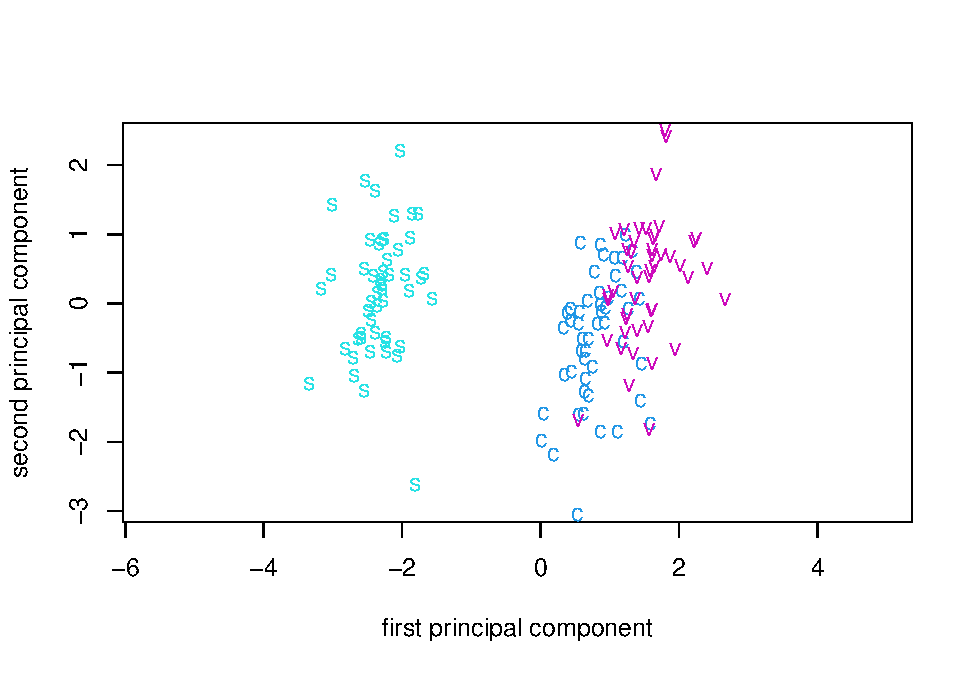
\includegraphics{modern_applied_statistics_CH11_files/figure-latex/unnamed-chunk-4-1.pdf}

\begin{Shaded}
\begin{Highlighting}[]
\FunctionTok{loadings}\NormalTok{(ir.pca)}
\end{Highlighting}
\end{Shaded}

\begin{verbatim}
## 
## Loadings:
##          Comp.1 Comp.2 Comp.3 Comp.4
## Sepal L.  0.504  0.455  0.709  0.191
## Sepal W. -0.302  0.889 -0.331       
## Petal L.  0.577        -0.219 -0.786
## Petal W.  0.567        -0.583  0.580
## 
##                Comp.1 Comp.2 Comp.3 Comp.4
## SS loadings      1.00   1.00   1.00   1.00
## Proportion Var   0.25   0.25   0.25   0.25
## Cumulative Var   0.25   0.50   0.75   1.00
\end{verbatim}

\begin{Shaded}
\begin{Highlighting}[]
\NormalTok{ir.pc }\OtherTok{\textless{}{-}} \FunctionTok{predict}\NormalTok{(ir.pca)}
\FunctionTok{eqscplot}\NormalTok{(ir.pc[, }\DecValTok{1}\SpecialCharTok{:}\DecValTok{2}\NormalTok{], }\AttributeTok{type =} \StringTok{"n"}\NormalTok{,}
         \AttributeTok{xlab =} \StringTok{"first principal component"}\NormalTok{,}
         \AttributeTok{ylab =} \StringTok{"second principal component"}\NormalTok{)}
\FunctionTok{text}\NormalTok{(ir.pc[, }\DecValTok{1}\SpecialCharTok{:}\DecValTok{2}\NormalTok{], }\AttributeTok{labels =} \FunctionTok{as.character}\NormalTok{(ir.species),}
     \AttributeTok{col =} \DecValTok{3} \SpecialCharTok{+} \FunctionTok{as.integer}\NormalTok{(ir.species)) }
\end{Highlighting}
\end{Shaded}

\includegraphics{modern_applied_statistics_CH11_files/figure-latex/unnamed-chunk-4-2.pdf}

\begin{Shaded}
\begin{Highlighting}[]
\CommentTok{\# Leptograpsus variegatus crabs dat}
\NormalTok{lcrabs }\OtherTok{\textless{}{-}} \FunctionTok{log}\NormalTok{(crabs[,}\DecValTok{4}\SpecialCharTok{:}\DecValTok{8}\NormalTok{])}
\NormalTok{crabs.grp }\OtherTok{\textless{}{-}} \FunctionTok{factor}\NormalTok{(}\FunctionTok{c}\NormalTok{(}\StringTok{"B"}\NormalTok{, }\StringTok{"b"}\NormalTok{, }\StringTok{"O"}\NormalTok{, }\StringTok{"o"}\NormalTok{)[}\FunctionTok{rep}\NormalTok{(}\DecValTok{1}\SpecialCharTok{:}\DecValTok{4}\NormalTok{, }\AttributeTok{each =} \DecValTok{50}\NormalTok{)])}
\NormalTok{(lcrabs.pca }\OtherTok{\textless{}{-}} \FunctionTok{princomp}\NormalTok{(lcrabs))}
\end{Highlighting}
\end{Shaded}

\begin{verbatim}
## Call:
## princomp(x = lcrabs)
## 
## Standard deviations:
##      Comp.1      Comp.2      Comp.3      Comp.4      Comp.5 
## 0.516640451 0.074653581 0.047914392 0.024804021 0.009052189 
## 
##  5  variables and  200 observations.
\end{verbatim}

\begin{Shaded}
\begin{Highlighting}[]
\FunctionTok{loadings}\NormalTok{(lcrabs.pca)}
\end{Highlighting}
\end{Shaded}

\begin{verbatim}
## 
## Loadings:
##    Comp.1 Comp.2 Comp.3 Comp.4 Comp.5
## FL  0.452  0.157  0.438  0.752  0.114
## RW  0.387 -0.911                     
## CL  0.453  0.204 -0.371        -0.784
## CW  0.440        -0.672         0.591
## BD  0.497  0.315  0.458 -0.652  0.136
## 
##                Comp.1 Comp.2 Comp.3 Comp.4 Comp.5
## SS loadings       1.0    1.0    1.0    1.0    1.0
## Proportion Var    0.2    0.2    0.2    0.2    0.2
## Cumulative Var    0.2    0.4    0.6    0.8    1.0
\end{verbatim}

\begin{Shaded}
\begin{Highlighting}[]
\NormalTok{lcrabs.pc }\OtherTok{\textless{}{-}} \FunctionTok{predict}\NormalTok{(lcrabs.pca)}
\FunctionTok{dimnames}\NormalTok{(lcrabs.pc) }\OtherTok{\textless{}{-}} \FunctionTok{list}\NormalTok{(}\ConstantTok{NULL}\NormalTok{, }\FunctionTok{paste}\NormalTok{(}\StringTok{"PC"}\NormalTok{, }\DecValTok{1}\SpecialCharTok{:}\DecValTok{5}\NormalTok{, }\AttributeTok{sep =} \StringTok{""}\NormalTok{))}
\FunctionTok{eqscplot}\NormalTok{(lcrabs.pc[, }\DecValTok{1}\SpecialCharTok{:}\DecValTok{2}\NormalTok{], }\AttributeTok{type =} \StringTok{"n"}\NormalTok{,}
         \AttributeTok{xlab =} \StringTok{"first principal component"}\NormalTok{,}
         \AttributeTok{ylab =} \StringTok{"second principal component"}\NormalTok{)}
\FunctionTok{text}\NormalTok{(lcrabs.pc[, }\DecValTok{1}\SpecialCharTok{:}\DecValTok{2}\NormalTok{], }\AttributeTok{labels =} \FunctionTok{as.character}\NormalTok{(crabs.grp),}
     \AttributeTok{col =} \DecValTok{3} \SpecialCharTok{+} \FunctionTok{as.integer}\NormalTok{(crabs.grp)) }
\end{Highlighting}
\end{Shaded}

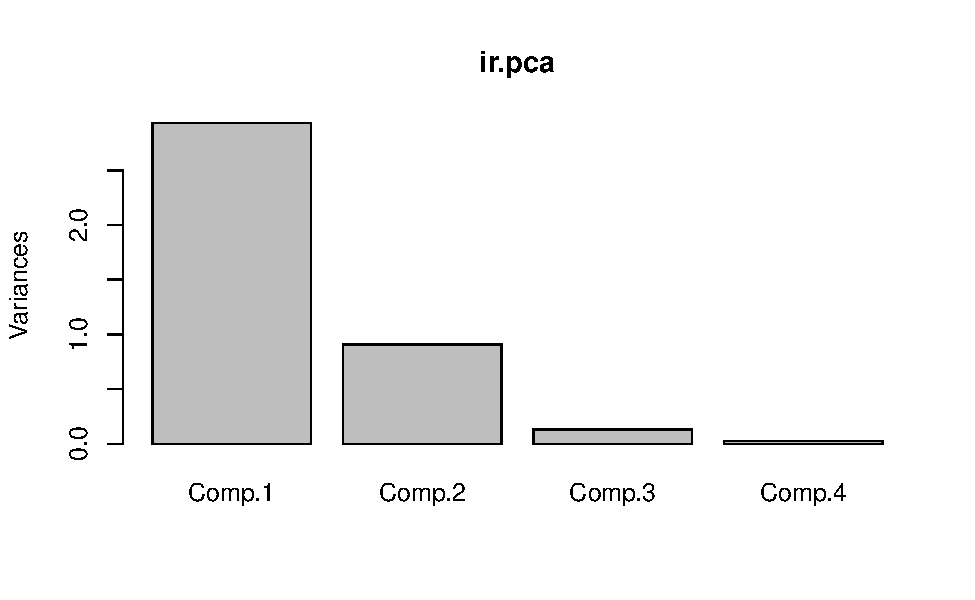
\includegraphics{modern_applied_statistics_CH11_files/figure-latex/unnamed-chunk-5-1.pdf}

\end{document}
